\subsection{Zustandshaltung der Pipeline}

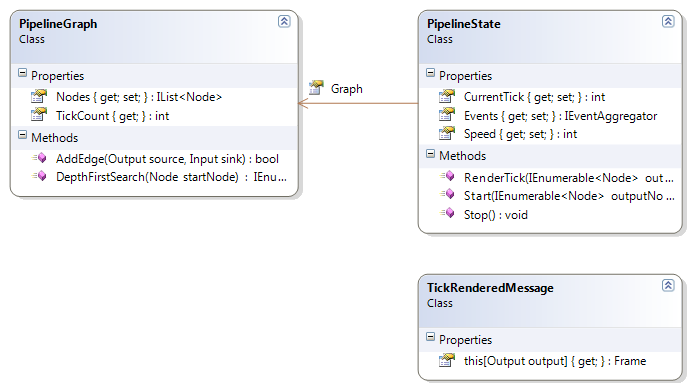
\includegraphics[width=\textwidth]{YuvKA.Pipeline/states.png}
Blablablubb PipelineState foo PipelineGraph bar.

\subsubsection{YuvKA.Pipeline.PipelineState}

\begin{verbatim}
[DataContract]
public class PipelineState
\end{verbatim}

\paragraph{Beschreibung}~\\
Die Klasse \name{PipelineState} vereint den gesamten Zustand des Datenmodells in sich, womit durch ihre Serialisierung die gesamten Programmdaten gespeichert werden. Sie enthält den aktuellen Wiedergabestatus und bietet zur Wiedergabe eine Schnittstelle zum \name{PipelineDriver}.

\paragraph{Typmember}
\begin{itemize}

\property{FrameIndex}
	\begin{verbatim}
	[DataMember]
	public int FrameIndex { get; set; }
	\end{verbatim}
	Ruft den Index des zuletzt angezeigten Frames ab oder legt ihn fest. Das Neusetzen führt nicht zum erneuten Berechnen des Frames, sondern muss mit \name{Start} explizit angefordert werden.

\property{Speed}
	\begin{verbatim}
	[DataMember]
	public int Speed { get; set; }
	\end{verbatim}
	Ruft die Abspielgeschwindigkeit in Frames pro Sekunde ab oder legt sie fest.

\method{Start}
	\begin{verbatim}
	public void Start()
	\end{verbatim}
	Weist den \name{PipelineDriver} an, die Pipeline ab dem aktuellen \name{FrameIndex} zu berechnen.

\method{Stop}
	\begin{verbatim}
	public void Stop()
	\end{verbatim}
	Beendet die Wiedergabe und stoppt den \name{PipelineDriver}. Danach vom \name{PipelineDriver} asynchron erhaltene Frames werden ignoriert.
\end{itemize}

\subsubsection{YuvKA.Pipeline.FrameRenderedMessage}

\subsubsection{YuvKA.Pipeline.PipelineGraph}
